\documentclass[12pt]{article}

\usepackage{tikz}

\title{algebraic-coding-theroy-part01}
\date{2022-11-26}
\author{XuGuoqiang}

\begin{document}

\maketitle

\section*{Introduction}

\begin{figure}[h!]
    \begin{center}
        \resizebox {!} {!} {
            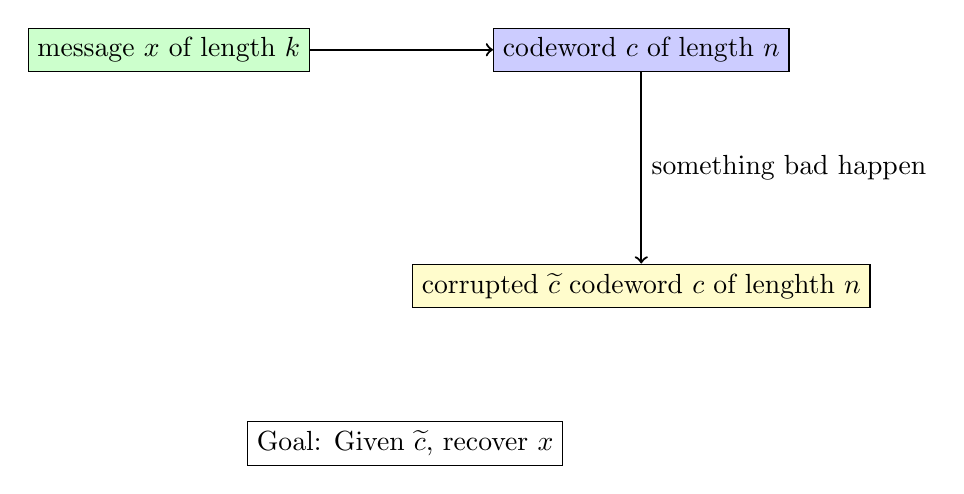
\begin{tikzpicture}
                \node(ori_m) at(-3, 0) [fill=green!20, draw]  {message $x$ of length $k$};
                \node(cod_m) at(3,  0) [fill=blue!20,  draw]  {codeword $c$ of length $n$};
                \node(rec_m) at(3,  -3) [fill=yellow!20, draw] {corrupted $\widetilde{c}$ codeword $c$ of lenghth $n$};
                \node(goal)  at(0, -5) [draw] {Goal: Given $\widetilde{c}$, recover $x$};
                \draw[thick]
                    [->] (ori_m) -- (cod_m);
                \draw[thick]
                    [->] (cod_m) -- node[right] {something bad happen} (rec_m);
            \end{tikzpicture}
        }
    \end{center}
\end{figure}

Examples:
\begin{itemize}
    \item Communication. Message corrupted in a noisy channel.
    \item Storage. SSD read, write, electrical, mechanical errors...
\end{itemize}

Goals:
\begin{itemize}
    \item Handling Something Bad
    \item Recovering Info About $x$
    \item Minimize Overhead, $\frac{k}{n}$ As Large As Possible
    \item Doing All The Things Efficiently Possible
\end{itemize}

Question: What is hand-off between all the goals?

\section*{Basics}

\begin{figure}[h!]
    \begin{center}
            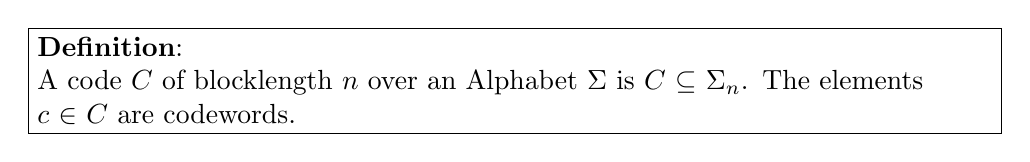
\begin{tikzpicture}
                \node[draw, text width=\textwidth, align=left] {\textbf{Definition}:\\A code $C$ of blocklength $n$ over an Alphabet $\Sigma$ is $C$ $\subseteq$ $\Sigma_{n}$.
                                         The elements \\$c$ $\in$ $C$ are codewords.};
            \end{tikzpicture}
    \end{center}
\end{figure}

Examples:
\begin{enumerate}
    \item $C=\{HELLOWORLD, BRUNCHTIME, ALLTHETIME\}$ is a code of blocklength 10 over $\Sigma = \{A, B, C, \dots, Z\}$.
    \item $ C=\left(\begin{array}{c c c c}
        0 & 0 & 0 & 0\\
        0 & 0 & 1 & 1\\
        0 & 1 & 0 & 1\\
        1 & 0 & 0 & 1\\
        1 & 0 & 1 & 0\\
        1 & 1 & 0 & 0\\
        1 & 1 & 1 & 1
    \end{array}\right)$ is a code of blocklength 4 over $\Sigma = \{0, 1\}$.
\end{enumerate}

\section*{Relation to Alice and Bob}

\begin{figure}[h!]
    \begin{center}
        \resizebox {!} {!} {
            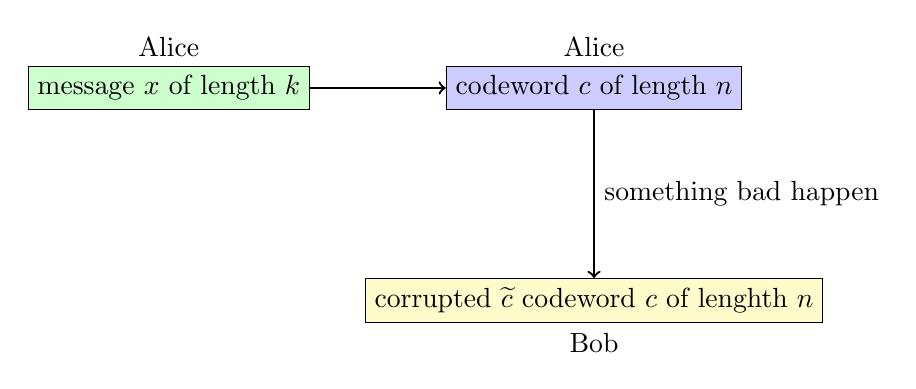
\begin{tikzpicture}[scale=0.9]
                \node(ori_m) at(-3, 0) [fill=green!20, draw, label=Alice]  {message $x$ of length $k$};
                \node(cod_m) at(3,  0) [fill=blue!20,  draw, label=Alice]  {codeword $c$ of length $n$};
                \node(rec_m) at(3,  -3) [fill=yellow!20, draw, label=below:Bob] {corrupted $\widetilde{c}$ codeword $c$ of lenghth $n$};
                \draw[thick]
                    [->] (ori_m) -- (cod_m);
                \draw[thick]
                    [->] (cod_m) -- node[right] {something bad happen} (rec_m);
            \end{tikzpicture}
        }
    \end{center}
\end{figure}

\newpage

Consider $ENC(\{0, 1\}^3) \mapsto \{0, 1\}^4$

\begin{figure}[h!]
    \begin{center}
            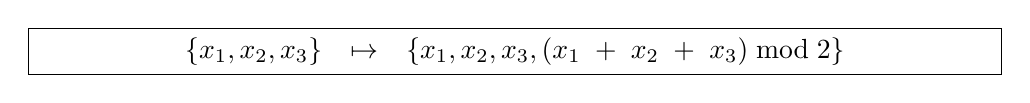
\begin{tikzpicture}
                \node[draw, text width=\textwidth, align=center] {$\{x_1, x_2, x_3\} \mapsto \{x_1, x_2, x_3, (x_1 + x_2 + x_3) \bmod 2 \}$};
            \end{tikzpicture}
    \end{center}
\end{figure}

Example: $ENC(\{0, 1, 1\}) = (0, 1, 1, 0)$
\vspace*{1\baselineskip}

This Code can correct one ERASURE.

Example: $(0, X, 0, 1)$. X must be 1.

\begin{figure}[h!]
    \begin{center}
            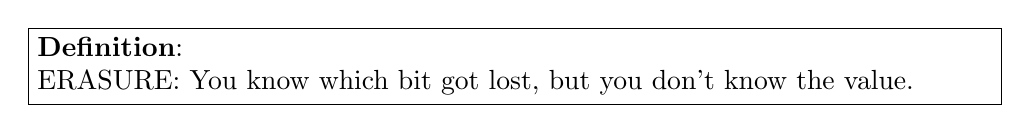
\begin{tikzpicture}
                \node[draw, text width=\textwidth, align=left] {\textbf{Definition}:\\ERASURE: You know which bit got lost, but you don't know the value.};
            \end{tikzpicture}
    \end{center}
\end{figure}

This Code can detect one ERROR.

Example: $(0, 0, 0, 1)$

\begin{figure}[h!]
    \begin{center}
            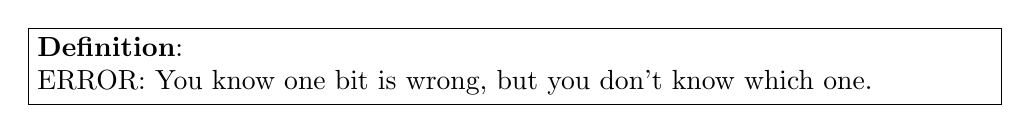
\begin{tikzpicture}
                \node[draw, text width=\textwidth, align=left] {\textbf{Definition}:\\ERROR: You know one bit is wrong, but you don't know which one.};
            \end{tikzpicture}
    \end{center}
\end{figure}

\subsubsection*{More Definitions}

\begin{figure}[h!]
    \begin{center}
            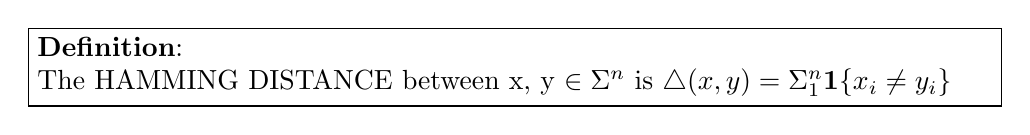
\begin{tikzpicture}
                \node[draw, text width=\textwidth, align=left] {\textbf{Definition}:\\The HAMMING DISTANCE between x, y $\in \Sigma^n$ is
                $\bigtriangleup(x, y)=\Sigma_1^n\mathbf{1}\{x_i \neq y_i\}$};
            \end{tikzpicture}
    \end{center}
\end{figure}

\end{document}